\documentclass[12pt,a4paper]{article}
\usepackage[UTF8]{ctex}
\usepackage{graphicx,geometry,amsmath,amssymb,listings,xcolor,float,fancyhdr,setspace}
\usepackage[most]{tcolorbox}

\newcommand{\fillin}[1]{\underline{\makebox[8cm][l]{#1}}}
\geometry{left=2.5cm,right=2.5cm,top=3.5cm,bottom=2.5cm}
\setlength{\headheight}{24.64995pt}

\pagestyle{fancy}
\fancyhf{}
\fancyhead[C]{\textbf{作业3 圆与多边形填充算法}}
\fancyhead[R]{\thepage}
\renewcommand{\headrulewidth}{2pt}

\lstdefinelanguage{Rust}{
    keywords={fn,let,mut,pub,struct,impl,for,if,else,while,return,use},
    keywords=[2]{i32,f64,bool,Vec,Self},
    sensitive=true,
    morecomment=[l]{//},
    morestring=[b]"
}

\lstset{
    language=Rust,
    basicstyle=\ttfamily\small,
    keywordstyle=\color{blue}\bfseries,
    keywordstyle=[2]\color{purple},
    commentstyle=\color{green!50!black},
    numbers=left,
    numberstyle=\tiny\color{gray},
    backgroundcolor=\color{gray!10},
    frame=single,
    breaklines=true
}

\begin{document}

\begin{titlepage}
\thispagestyle{empty}
\centering
\vspace*{10mm}
{\zihao{4} 《计算机图形学及人机交互》\par}
\vspace{20mm}
{\bfseries\zihao{1} 作 业 报 告\par}
\vspace{40mm}
\songti\zihao{-3}
\begin{flushleft}
\renewcommand\arraystretch{2}
\begin{tabular}{ll}
学\quad 号： & \fillin{2023112621} \\
姓\quad 名： & \fillin{程泽凯} \\
年\quad 级： & \fillin{2023 级} \\
专\quad 业： & \fillin{计算机科学与技术} \\
院\quad 系： & \fillin{计算机与人工智能学院} \\
\end{tabular}
\end{flushleft}
\vfill
{\zihao{-3} 2024~2025 第 1 学期\par}
\end{titlepage}

\clearpage
\tableofcontents
\clearpage

\songti\zihao{-4}
\onehalfspacing

\section{Bresenham圆绘制算法（40分）}

\subsection{算法文字描述（15分）}

\begin{tcolorbox}[breakable]
\textbf{算法思想：}

Bresenham圆绘制算法是一种增量式整数运算算法，通过利用圆的对称性和整数判别式来高效地绘制圆。该算法避免了浮点运算和复杂的平方根计算，仅使用加法和位移操作。

\textbf{1. 圆的隐式方程}

对于圆心在 $(x_c, y_c)$、半径为 $r$ 的圆，其隐式方程为：
\begin{equation}
F(x,y) = (x-x_c)^2 + (y-y_c)^2 - r^2 = 0
\end{equation}

为简化分析，考虑圆心在原点的圆：$F(x,y) = x^2 + y^2 - r^2 = 0$

\textbf{2. 八分对称性}

圆具有八分对称性，即：
\begin{itemize}
\item 关于x轴对称：$(x,y) \leftrightarrow (x,-y)$
\item 关于y轴对称：$(x,y) \leftrightarrow (-x,y)$
\item 关于原点对称：$(x,y) \leftrightarrow (-x,-y)$
\item 关于直线 $y=x$ 对称：$(x,y) \leftrightarrow (y,x)$
\end{itemize}

因此，只需计算第一个八分圆（从$(0,r)$到$(r/\sqrt{2}, r/\sqrt{2})$，即$0° \sim 45°$）上的点，其余7个八分圆上的点可通过对称变换得到。在此区间内，满足 $x \leq y$。

\textbf{3. 决策参数推导}

在绘制过程中，假设当前点为 $(x_k, y_k)$，下一个点有两种选择：
\begin{itemize}
\item $P_1 = (x_k+1, y_k)$：水平向右移动
\item $P_2 = (x_k+1, y_k-1)$：右下移动
\end{itemize}

引入决策参数 $d_k$ 来判断选择哪个点：
\begin{equation}
d_k = F(x_k+1, y_k-0.5) = (x_k+1)^2 + (y_k-0.5)^2 - r^2
\end{equation}

\begin{itemize}
\item 若 $d_k < 0$：说明中点在圆内，实际圆弧离 $P_1$ 更近，选择 $P_1$，即 $y$ 不变
\item 若 $d_k \geq 0$：说明中点在圆外，实际圆弧离 $P_2$ 更近，选择 $P_2$，即 $y$ 减1
\end{itemize}

\textbf{4. 决策参数的增量计算}

\textbf{（1）初始值推导}

当 $x_0=0, y_0=r$ 时，需要计算第一个中点 $(1, r-0.5)$ 的决策参数：
\begin{align}
d_0 &= F(1, r-0.5) \\
&= 1^2 + (r-0.5)^2 - r^2 \\
&= 1 + r^2 - r + 0.25 - r^2 \\
&= 1.25 - r
\end{align}

为避免浮点数运算，我们可以：
\begin{itemize}
\item 将决策参数乘以2：$d_0' = 2d_0 = 2.5 - 2r \approx 2 - 2r$
\item 或者使用近似：$d_0 = 1 - r$
\item \textbf{实际使用：}$d_0 = 3 - 2r$（整数，便于计算）
\end{itemize}

\textbf{（2）增量更新推导}

决策参数的更新采用增量方式，避免重复计算。

\textbf{情况1：}若 $d_k < 0$（选择$P_1 = (x_k+1, y_k)$，水平右移）

下一个中点为 $(x_k+2, y_k-0.5)$，计算 $d_{k+1}$：
\begin{align}
d_{k+1} &= F(x_k+2, y_k-0.5) \\
&= (x_k+2)^2 + (y_k-0.5)^2 - r^2 \\
&= \left[(x_k+1)^2 + (y_k-0.5)^2 - r^2\right] + 2(x_k+1) + 1 \\
&= d_k + 2(x_k+1) + 1 \\
&= d_k + 2x_k + 3
\end{align}

若使用 $2d$ 形式（决策参数乘以2），则：
\begin{equation}
\boxed{d_{k+1} = d_k + 4x_k + 6}
\end{equation}

\textbf{情况2：}若 $d_k \geq 0$（选择$P_2 = (x_k+1, y_k-1)$，右下移动）

下一个中点为 $(x_k+2, y_k-1.5)$，计算 $d_{k+1}$：
\begin{align}
d_{k+1} &= F(x_k+2, y_k-1.5) \\
&= (x_k+2)^2 + (y_k-1.5)^2 - r^2 \\
&= \left[(x_k+1)^2 + (y_k-0.5)^2 - r^2\right] + 2(x_k+1) + 1 - 2y_k + 1 \\
&= d_k + 2(x_k+1) + 1 - 2y_k + 1 \\
&= d_k + 2(x_k - y_k + 1) + 2 \\
&= d_k + 2x_k - 2y_k + 4
\end{align}

若使用 $2d$ 形式，则：
\begin{equation}
\boxed{d_{k+1} = d_k + 4(x_k - y_k) + 10}
\end{equation}

\textbf{（3）增量计算总结}

\begin{center}
\begin{tabular}{|l|c|c|}
\hline
\textbf{条件} & \textbf{选择的点} & \textbf{决策参数更新} \\
\hline
$d_k < 0$ & $(x_k+1, y_k)$ & $d_{k+1} = d_k + 4x_k + 6$ \\
\hline
$d_k \geq 0$ & $(x_k+1, y_k-1)$ & $d_{k+1} = d_k + 4(x_k-y_k) + 10$ \\
\hline
\end{tabular}
\end{center}

\vspace{3mm}

\textbf{5. 算法流程}

\textbf{完整的Bresenham圆绘制算法步骤如下：}

\begin{enumerate}
\item \textbf{初始化：}
  \begin{itemize}
  \item $x = 0$，$y = r$
  \item $d = 3 - 2r$
  \end{itemize}

\item \textbf{循环绘制}（当 $x \leq y$ 时）：
  \begin{itemize}
  \item 根据当前点 $(x, y)$ 绘制8个对称点：
    \begin{align*}
    &(x_c+x, y_c+y), \quad (x_c+y, y_c+x) \\
    &(x_c-x, y_c+y), \quad (x_c-y, y_c+x) \\
    &(x_c+x, y_c-y), \quad (x_c+y, y_c-x) \\
    &(x_c-x, y_c-y), \quad (x_c-y, y_c-x)
    \end{align*}
  \item 判断并更新：
    \begin{itemize}
    \item 若 $d < 0$：$d \leftarrow d + 4x + 6$
    \item 若 $d \geq 0$：$d \leftarrow d + 4(x-y) + 10$，$y \leftarrow y - 1$
    \end{itemize}
  \item $x \leftarrow x + 1$
  \end{itemize}

\item \textbf{终止条件：}当 $x > y$ 时停止（已完成第一个八分圆）
\end{enumerate}

\vspace{3mm}

\textbf{6. 算法特点与复杂度分析}

\begin{itemize}
\item \textbf{优点：}
  \begin{itemize}
  \item 仅使用整数加法和位移运算，速度快
  \item 利用对称性，只需计算1/8圆周，生成8倍的点
  \item 避免了浮点运算和三角函数计算
  \item 误差控制在1个像素以内
  \end{itemize}
  
\item \textbf{缺点：}
  \begin{itemize}
  \item 仅适用于标准圆，不能直接用于椭圆
  \item 需要特殊处理对称点的重复问题
  \end{itemize}

\item \textbf{复杂度分析：}
  \begin{itemize}
  \item \textbf{时间复杂度：}$O(r)$，其中 $r$ 是圆的半径。只需遍历第一个八分圆的 $r/\sqrt{2}$ 个点。
  \item \textbf{空间复杂度：}$O(1)$，仅需要常数个变量存储当前状态。
  \end{itemize}

\item \textbf{应用场景：}
  \begin{itemize}
  \item 计算机图形学中的圆形绘制
  \item 游戏开发中的碰撞检测
  \item CAD系统中的圆形对象渲染
  \end{itemize}
\end{itemize}
\end{tcolorbox}

\subsection{计算示例（10分）}

\textbf{问题：}圆心(2,2)，半径10，求x=8时的y值

\textbf{理论验证：}$(8-2)^2+(y-2)^2=100 \Rightarrow y=10$ 或 $y=-6$

\textbf{Bresenham计算过程：}

\textbf{初始化：}
\begin{align*}
x &= 0 \\
y &= r = 10 \\
d &= 3 - 2r = 3 - 2 \times 10 = -17
\end{align*}

\textbf{详细迭代过程：}

下面逐步展示每次迭代的完整计算过程，包括决策判断、参数更新、几何意义和验证。

\begin{enumerate}
\item \textbf{第1次迭代}（$x=0, y=10$）：
  \begin{itemize}
  \item \textbf{当前点：}$(x, y) = (0, 10)$，相对圆心的坐标
  \item \textbf{绝对坐标：}$(x_c + x, y_c + y) = (2, 12)$
  \item \textbf{决策参数：}$d = -17$
  \item \textbf{中点坐标：}$(x+1, y-0.5) = (1, 9.5)$
  \item \textbf{中点判断：}$d = F(1, 9.5) = 1^2 + 9.5^2 - 10^2 = 1 + 90.25 - 100 = -8.75 < 0$
    
    说明中点在圆内，选择 $P_1 = (1, 10)$（水平右移）
  \item \textbf{决策：}$d < 0$，使用增量公式 $d_{new} = d + 4x + 6$
  \item \textbf{参数更新：}
    \begin{align*}
    d_{new} &= -17 + 4 \times 0 + 6 = -17 + 0 + 6 = -11 \\
    x_{new} &= 0 + 1 = 1 \\
    y_{new} &= 10 \text{（不变）}
    \end{align*}
  \item \textbf{点验证：}$x^2 + y^2 = 0^2 + 10^2 = 100 = r^2$ \checkmark（精确在圆上）
  \item \textbf{继续条件：}$x = 0 \leq y = 10$ \checkmark
  \end{itemize}

\item \textbf{第2次迭代}（$x=1, y=10$）：
  \begin{itemize}
  \item \textbf{当前点：}$(1, 10)$
  \item \textbf{绝对坐标：}$(3, 12)$
  \item \textbf{决策参数：}$d = -11$
  \item \textbf{中点坐标：}$(2, 9.5)$
  \item \textbf{中点判断：}$F(2, 9.5) = 4 + 90.25 - 100 = -5.75 < 0$
    
    中点在圆内，选择 $(2, 10)$
  \item \textbf{决策：}$d = -11 < 0$
  \item \textbf{参数更新：}
    \begin{align*}
    d_{new} &= -11 + 4 \times 1 + 6 = -11 + 4 + 6 = -1 \\
    x_{new} &= 1 + 1 = 2 \\
    y_{new} &= 10
    \end{align*}
  \item \textbf{点验证：}$1^2 + 10^2 = 101 \approx 100$（误差1，接近圆）
  \item \textbf{继续条件：}$x = 1 \leq y = 10$ \checkmark
  \end{itemize}

\item \textbf{第3次迭代}（$x=2, y=10$）：
  \begin{itemize}
  \item \textbf{当前点：}$(2, 10)$
  \item \textbf{绝对坐标：}$(4, 12)$
  \item \textbf{决策参数：}$d = -1$
  \item \textbf{中点坐标：}$(3, 9.5)$
  \item \textbf{中点判断：}$F(3, 9.5) = 9 + 90.25 - 100 = -0.75 < 0$
    
    中点在圆内（接近边界），选择 $(3, 10)$
  \item \textbf{决策：}$d = -1 < 0$
  \item \textbf{参数更新：}
    \begin{align*}
    d_{new} &= -1 + 4 \times 2 + 6 = -1 + 8 + 6 = 13 \\
    x_{new} &= 2 + 1 = 3 \\
    y_{new} &= 10
    \end{align*}
  \item \textbf{点验证：}$2^2 + 10^2 = 104 \approx 100$（误差4）
  \item \textbf{继续条件：}$x = 2 \leq y = 10$ \checkmark
  \end{itemize}

\item \textbf{第4次迭代}（$x=3, y=10$）：
  \begin{itemize}
  \item \textbf{当前点：}$(3, 10)$
  \item \textbf{绝对坐标：}$(5, 12)$
  \item \textbf{决策参数：}$d = 13$
  \item \textbf{中点坐标：}$(4, 9.5)$
  \item \textbf{中点判断：}$F(4, 9.5) = 16 + 90.25 - 100 = 6.25 > 0$
    
    中点在圆外，选择 $P_2 = (4, 9)$（右下移动）
  \item \textbf{决策：}$d = 13 \geq 0$，使用增量公式 $d_{new} = d + 4(x-y) + 10$
  \item \textbf{参数更新：}
    \begin{align*}
    d_{new} &= 13 + 4 \times (3-10) + 10 \\
    &= 13 + 4 \times (-7) + 10 \\
    &= 13 - 28 + 10 = -5 \\
    y_{new} &= 10 - 1 = 9 \\
    x_{new} &= 3 + 1 = 4
    \end{align*}
  \item \textbf{点验证：}$3^2 + 10^2 = 109 \neq 100$（误差较大，但下一个点会更接近）
  \item \textbf{继续条件：}$x = 3 \leq y = 10$ \checkmark
  \end{itemize}

\item \textbf{第5次迭代}（$x=4, y=9$）：
  \begin{itemize}
  \item \textbf{当前点：}$(4, 9)$
  \item \textbf{绝对坐标：}$(6, 11)$
  \item \textbf{决策参数：}$d = -5$
  \item \textbf{中点坐标：}$(5, 8.5)$
  \item \textbf{中点判断：}$F(5, 8.5) = 25 + 72.25 - 100 = -2.75 < 0$
    
    中点在圆内，选择 $(5, 9)$
  \item \textbf{决策：}$d = -5 < 0$
  \item \textbf{参数更新：}
    \begin{align*}
    d_{new} &= -5 + 4 \times 4 + 6 = -5 + 16 + 6 = 17 \\
    x_{new} &= 4 + 1 = 5 \\
    y_{new} &= 9
    \end{align*}
  \item \textbf{点验证：}$4^2 + 9^2 = 16 + 81 = 97 \approx 100$（误差3）
  \item \textbf{继续条件：}$x = 4 \leq y = 9$ \checkmark
  \end{itemize}

\item \textbf{第6次迭代}（$x=5, y=9$）：
  \begin{itemize}
  \item \textbf{当前点：}$(5, 9)$
  \item \textbf{绝对坐标：}$(7, 11)$
  \item \textbf{决策参数：}$d = 17$
  \item \textbf{中点坐标：}$(6, 8.5)$
  \item \textbf{中点判断：}$F(6, 8.5) = 36 + 72.25 - 100 = 8.25 > 0$
    
    中点在圆外，选择 $(6, 8)$
  \item \textbf{决策：}$d = 17 \geq 0$
  \item \textbf{参数更新：}
    \begin{align*}
    d_{new} &= 17 + 4 \times (5-9) + 10 \\
    &= 17 + 4 \times (-4) + 10 \\
    &= 17 - 16 + 10 = 11 \\
    y_{new} &= 9 - 1 = 8 \\
    x_{new} &= 5 + 1 = 6
    \end{align*}
  \item \textbf{点验证：}$5^2 + 9^2 = 25 + 81 = 106 \neq 100$（误差6）
  \item \textbf{继续条件：}$x = 5 \leq y = 9$ \checkmark
  \end{itemize}

\item \textbf{第7次迭代}（$x=6, y=8$）：
  \begin{itemize}
  \item \textbf{当前点：}$(6, 8)$
  \item \textbf{绝对坐标：}$(8, 10)$ \quad \textcolor{red}{← 这是我们要找的点！}
  \item \textbf{决策参数：}$d = 11$
  \item \textbf{中点坐标：}$(7, 7.5)$
  \item \textbf{中点判断：}$F(7, 7.5) = 49 + 56.25 - 100 = 5.25 > 0$
    
    中点在圆外，选择 $(7, 7)$
  \item \textbf{决策：}$d = 11 \geq 0$
  \item \textbf{参数更新：}
    \begin{align*}
    d_{new} &= 11 + 4 \times (6-8) + 10 \\
    &= 11 + 4 \times (-2) + 10 \\
    &= 11 - 8 + 10 = 13 \\
    y_{new} &= 8 - 1 = 7 \\
    x_{new} &= 6 + 1 = 7
    \end{align*}
  \item \textbf{点验证：}$6^2 + 8^2 = 36 + 64 = 100 = r^2$ \checkmark（精确在圆上！）
  \item \textbf{继续条件：}$x = 6 \leq y = 8$ \checkmark
  \end{itemize}

\item \textbf{第8次迭代}（$x=7, y=7$）：
  \begin{itemize}
  \item \textbf{当前点：}$(7, 7)$
  \item \textbf{绝对坐标：}$(9, 9)$
  \item \textbf{决策参数：}$d = 13$
  \item \textbf{点验证：}$7^2 + 7^2 = 49 + 49 = 98 \approx 100$（误差2）
  \item \textbf{终止判断：}$x = 7 \leq y = 7$（边界情况），可以继续一次或终止
  \item 如果继续：$x_{new} = 8 > y = 7$ 或 $y_{new} = 6$，满足 $x > y$，\textbf{终止}
  \end{itemize}
\end{enumerate}

\vspace{5mm}
\textbf{迭代过程汇总表：}

\begin{table}[H]
\centering
\small
\begin{tabular}{|c|c|c|c|c|c|c|c|}
\hline
\textbf{迭代} & \textbf{$x$} & \textbf{$y$} & \textbf{$d$} & \textbf{决策} & \textbf{$d_{new}$} & \textbf{绝对坐标} & \textbf{$x^2+y^2$} \\
\hline
初始 & 0 & 10 & -17 & - & - & (2,12) & 100 \\
\hline
1 & 0 & 10 & -17 & $d<0$ & -11 & (2,12) & 100 \\
\hline
2 & 1 & 10 & -11 & $d<0$ & -1 & (3,12) & 101 \\
\hline
3 & 2 & 10 & -1 & $d<0$ & 13 & (4,12) & 104 \\
\hline
4 & 3 & 10 & 13 & $d\geq 0$ & -5 & (5,12) & 109 \\
\hline
5 & 4 & 9 & -5 & $d<0$ & 17 & (6,11) & 97 \\
\hline
6 & 5 & 9 & 17 & $d\geq 0$ & 11 & (7,11) & 106 \\
\hline
7 & 6 & 8 & 11 & $d\geq 0$ & 13 & \textcolor{red}{(8,10)} & \textcolor{red}{100} \\
\hline
8 & 7 & 7 & 13 & 终止 & - & (9,9) & 98 \\
\hline
\end{tabular}
\caption{Bresenham圆算法迭代过程汇总（圆心(2,2)，半径10）}
\end{table}

\textbf{关键观察：}
\begin{itemize}
\item 第1次和第7次迭代得到的点 $(0,10)$ 和 $(6,8)$ 精确在圆上（$x^2+y^2=100$）
\item 其他点都是近似点，但误差很小（最大误差9，相对误差9\%）
\item 决策参数 $d$ 在正负之间交替变化，反映了实际圆弧在候选点之间的位置
\item 当 $d$ 从负变正时（第4、6次迭代），算法选择向下移动，使点更接近圆弧
\end{itemize}

\textbf{利用八分对称性求解：}

根据圆的八分对称性，对于第一象限内的点 $(x_0, y_0)$，可以得到8个对称点：
\begin{align*}
&(x_c + x_0, y_c + y_0), \quad (x_c + y_0, y_c + x_0) \\
&(x_c - x_0, y_c + y_0), \quad (x_c - y_0, y_c + x_0) \\
&(x_c + x_0, y_c - y_0), \quad (x_c + y_0, y_c - x_0) \\
&(x_c - x_0, y_c - y_0), \quad (x_c - y_0, y_c - x_0)
\end{align*}

当 $x_0 = 6, y_0 = 8$ 时（圆心为$(2,2)$）：
\begin{align*}
&(2+6, 2+8) = (8, 10) \quad \checkmark \\
&(2+8, 2+6) = (10, 8) \\
&(2-6, 2+8) = (-4, 10) \\
&(2-8, 2+6) = (-6, 8) \\
&(2+6, 2-8) = (8, -6) \quad \checkmark \\
&(2+8, 2-6) = (10, -4) \\
&(2-6, 2-8) = (-4, -6) \\
&(2-8, 2-6) = (-6, -4)
\end{align*}

因此，当 $x=8$ 时，得到 $y=10$ 或 $y=-6$。

\textbf{结论：}$\boxed{y=10\text{ 或 }y=-6}$

\subsection{Rust实现（15分）}

\begin{lstlisting}
pub fn bresenham_circle(cx: i32, cy: i32, r: i32) -> Vec<Point> {
    let mut points = Vec::new();
    let (mut x, mut y) = (0, r);
    let mut d = 3 - 2 * r;
    
    while x <= y {
        // 8个对称点
        points.push(Point::new(cx+x, cy+y));
        points.push(Point::new(cx+y, cy+x));
        points.push(Point::new(cx-x, cy+y));
        points.push(Point::new(cx-y, cy+x));
        points.push(Point::new(cx-x, cy-y));
        points.push(Point::new(cx-y, cy-x));
        points.push(Point::new(cx+x, cy-y));
        points.push(Point::new(cx+y, cy-x));
        
        if d < 0 {
            d += 4 * x + 6;
        } else {
            d += 4 * (x - y) + 10;
            y -= 1;
        }
        x += 1;
    }
    points
}
\end{lstlisting}

\section{多边形填充算法（60分）}

\subsection{扫描线填充算法}

\subsubsection{算法描述（10分）}

\begin{tcolorbox}[breakable]
\textbf{算法思想：}

扫描线填充算法是一种基于扫描线的区域填充算法，通过水平扫描线从下到上逐行扫描多边形，计算扫描线与多边形边的交点，然后在交点间进行配对填充。该算法高效且适用于任意复杂的多边形。

\textbf{1. 核心数据结构}

\textbf{（1）边表（Edge Table, ET）}

边表是一个按扫描线 $y$ 坐标组织的数组，$ET[y]$ 存储 $y_{min} = y$ 的所有非水平边。每条边记录以下信息：
\begin{itemize}
\item $y_{max}$：边的最大 $y$ 坐标
\item $x$：边与当前扫描线的交点的 $x$ 坐标
\item $\Delta x$：扫描线每增加1时，交点 $x$ 坐标的增量（即斜率的倒数 $1/k$）
\end{itemize}

边的结构体表示为：
\begin{verbatim}
struct Edge {
    y_max: i32,      // 边的上端点y坐标
    x: f64,          // 当前扫描线交点的x坐标
    dx: f64,         // 斜率的倒数 1/k
}
\end{verbatim}

\textbf{（2）活性边表（Active Edge Table, AET）}

活性边表存储与当前扫描线相交的所有边，按照交点的 $x$ 坐标递增排序。AET中的边满足：
\begin{equation}
y_{min} \leq y_{current} < y_{max}
\end{equation}

\textbf{2. 算法详细步骤}

\textbf{步骤1：构造边表ET}

遍历多边形的所有顶点，对于每条边 $(v_i, v_{i+1})$：
\begin{enumerate}
\item 跳过水平边（$y_i = y_{i+1}$）
\item 确定边的下端点 $y_{min}$ 和上端点 $y_{max}$
\item 计算斜率倒数：$\Delta x = \frac{x_{i+1} - x_i}{y_{i+1} - y_i}$
\item 将边信息插入 $ET[y_{min}]$ 中
\end{enumerate}

\textbf{特殊处理：}对于顶点，若该顶点是多边形的局部极值点（如局部最大值或最小值），则只计入一条边；若是普通顶点，需要正确处理以避免重复计数。

\textbf{步骤2：初始化扫描}

\begin{itemize}
\item 找到多边形的最小 $y$ 坐标：$y = y_{min}$
\item 初始化活性边表 $AET = \emptyset$
\end{itemize}

\textbf{步骤3：扫描线循环}（从 $y_{min}$ 到 $y_{max}$）

对于每条扫描线 $y$，执行以下操作：

\textbf{（1）更新AET}
\begin{itemize}
\item 将 $ET[y]$ 中的所有边加入 $AET$
\item 从 $AET$ 中删除满足 $y \geq y_{max}$ 的边（这些边已经处理完毕）
\item 按 $x$ 坐标对 $AET$ 进行排序
\end{itemize}

\textbf{（2）填充像素}

采用奇偶规则（Odd-Even Rule）或非零环绕数规则（Non-Zero Winding Rule）进行填充：
\begin{itemize}
\item \textbf{奇偶规则：}从左到右扫描 $AET$，交点配对填充。第1和第2个交点之间填充，第3和第4个交点之间填充，依此类推。
\item 具体实现：按顺序取 $AET$ 中相邻的交点对 $(x_i, x_{i+1})$（$i$ 为奇数），填充区间 $[\lceil x_i \rceil, \lfloor x_{i+1} \rfloor]$ 内的所有像素。
\end{itemize}

\textbf{（3）更新交点x坐标}

对于 $AET$ 中的每条边，更新其与下一条扫描线的交点：
\begin{equation}
x_{new} = x_{old} + \Delta x
\end{equation}

\textbf{步骤4：终止条件}

当 $y > y_{max}$ 且 $AET$ 为空时，算法结束。

\textbf{3. 边界情况处理}

\begin{itemize}
\item \textbf{水平边：}不加入边表，因为水平边对填充没有贡献
\item \textbf{共享顶点：}对于共享顶点，使用"下闭上开"原则，即边的下端点包含在边中，上端点不包含，避免顶点被重复处理
\item \textbf{退化多边形：}处理面积为0的多边形（如共线点）
\end{itemize}

\textbf{4. 算法特点}

\begin{itemize}
\item \textbf{优点：}
  \begin{itemize}
  \item 利用扫描线的连贯性，避免重复计算
  \item 仅需要维护活性边，空间效率高
  \item 适用于复杂多边形和带孔多边形
  \end{itemize}
\item \textbf{缺点：}
  \begin{itemize}
  \item 需要构造和维护边表，实现相对复杂
  \item 需要对AET进行排序，有一定的开销
  \end{itemize}
\item \textbf{时间复杂度：}$O(n + h \cdot (e \log e + w))$
  \begin{itemize}
  \item $n$：多边形顶点数
  \item $h$：多边形高度（扫描线数量）
  \item $e$：平均每条扫描线相交的边数
  \item $w$：每条扫描线填充的像素宽度
  \end{itemize}
\item \textbf{空间复杂度：}$O(n + e)$
\end{itemize}
\end{tcolorbox}

\subsubsection{Rust实现（15分）}

\begin{lstlisting}
pub fn scanline_fill(vertices: &[Point]) -> Vec<Point> {
    let mut points = Vec::new();
    let y_min = vertices.iter().map(|p| p.y).min().unwrap();
    let y_max = vertices.iter().map(|p| p.y).max().unwrap();
    
    // 构建边表...
    // 扫描线填充...
    
    for y in y_min..=y_max {
        // 加入新边，排序，配对填充，更新AET
    }
    points
}
\end{lstlisting}

\subsubsection{复杂度分析（5分）}

\textbf{时间复杂度详细分析：}

我们逐步分析算法各部分的时间开销：

\textbf{1. 构造边表ET}
\begin{lstlisting}[language=Rust, numbers=none]
// 遍历所有顶点，构造边表
for i in 0..n {                              // O(n)
    let edge = (vertices[i], vertices[(i+1) % n]);
    if edge.y_min != edge.y_max {            // 跳过水平边
        ET[edge.y_min].push(edge);           // O(1) 插入
    }
}
\end{lstlisting}
\textbf{时间：}$O(n)$，其中 $n$ 为顶点数（即边数）

\textbf{2. 扫描线循环}
\begin{lstlisting}[language=Rust, numbers=none]
for y in y_min..=y_max {                     // O(h) 循环h次
    // (a) 更新AET：加入新边
    AET.extend(ET[y]);                       // O(e_y) 加入e_y条新边
    
    // (b) 删除失效的边
    AET.retain(|edge| edge.y_max > y);       // O(e) 遍历AET
    
    // (c) 对AET按x坐标排序
    AET.sort_by(|a, b| a.x.cmp(&b.x));       // O(e log e)
    
    // (d) 配对填充
    for i in (0..AET.len()).step_by(2) {     // O(w) 填充w个像素
        fill_line(AET[i].x, AET[i+1].x, y);
    }
    
    // (e) 更新交点x坐标
    for edge in &mut AET {                   // O(e)
        edge.x += edge.dx;
    }
}
\end{lstlisting}

每条扫描线的时间开销：
\begin{itemize}
\item 加入新边：$O(e_y)$，平均为 $O(e/h)$
\item 删除失效边：$O(e)$
\item 排序AET：$O(e \log e)$
\item 配对填充：$O(w)$，$w$ 为填充宽度
\item 更新交点：$O(e)$
\end{itemize}

单条扫描线总时间：$O(e \log e + w)$

\textbf{3. 总时间复杂度推导}
\begin{align}
T_{total} &= T_{构造ET} + T_{扫描} \\
&= O(n) + \sum_{y=y_{min}}^{y_{max}} O(e \log e + w) \\
&= O(n) + h \cdot O(e \log e + w) \\
&= O(n + h(e \log e + w))
\end{align}

其中：
\begin{itemize}
\item $n$：多边形边数
\item $h = y_{max} - y_{min} + 1$：扫描线数量（多边形高度）
\item $e$：平均每条扫描线的活性边数，通常 $e \ll n$
\item $w$：平均每条扫描线的填充宽度
\end{itemize}

\textbf{最坏情况：}对于复杂多边形，$e \approx n$，时间复杂度为 $O(n + h(n \log n + w))$

\textbf{最好情况：}对于简单凸多边形，$e = 2$（每条扫描线只与2条边相交），时间复杂度为 $O(n + h \cdot w)$

\vspace{3mm}
\textbf{空间复杂度分析：}

\begin{itemize}
\item 边表ET：存储所有非水平边，$O(n)$
\item 活性边表AET：存储当前扫描线的活性边，最坏情况 $O(e)$，其中 $e \leq n$
\item 其他辅助变量：$O(1)$
\end{itemize}

\textbf{总空间复杂度：}$S = O(n + e) = O(n)$

\subsection{栅栏填充算法}

\subsubsection{算法描述（10分）}

\begin{tcolorbox}[breakable]
\textbf{算法思想：}

栅栏填充算法（Fence Fill）是扫描线填充算法的简化版本，其核心思想是对每条扫描线，直接遍历多边形的所有边，计算与该扫描线的交点，然后对交点排序并配对填充。该算法不维护边表和活性边表，实现更加简单直观。

\textbf{1. 算法详细步骤}

\textbf{步骤1：确定扫描范围}

遍历多边形的所有顶点，找到最小和最大的 $y$ 坐标：
\begin{align}
y_{min} &= \min\{y_i \mid i = 1, 2, \ldots, n\} \\
y_{max} &= \max\{y_i \mid i = 1, 2, \ldots, n\}
\end{align}

\textbf{步骤2：扫描线循环}

对于每条扫描线 $y \in [y_{min}, y_{max}]$：

\textbf{（1）计算交点}

遍历多边形的所有边 $(v_i, v_{i+1})$，判断边是否与扫描线相交：
\begin{itemize}
\item 跳过水平边：$y_i = y_{i+1}$
\item 判断相交条件：$\min(y_i, y_{i+1}) \leq y < \max(y_i, y_{i+1})$（使用"下闭上开"原则）
\item 若相交，计算交点的 $x$ 坐标：
  \begin{equation}
  x = x_i + \frac{(y - y_i) \cdot (x_{i+1} - x_i)}{y_{i+1} - y_i}
  \end{equation}
\item 将 $x$ 加入交点列表
\end{itemize}

\textbf{（2）交点排序}

将交点列表按 $x$ 坐标递增排序：
\begin{equation}
\text{sort}(\{x_1, x_2, \ldots, x_k\}) \rightarrow \{x'_1, x'_2, \ldots, x'_k\} \quad \text{其中} \quad x'_1 \leq x'_2 \leq \cdots \leq x'_k
\end{equation}

\textbf{（3）配对填充}

按照奇偶规则进行填充：
\begin{itemize}
\item 将交点两两配对：$(x'_1, x'_2), (x'_3, x'_4), \ldots, (x'_{k-1}, x'_k)$（假设 $k$ 为偶数）
\item 对每一对 $(x'_i, x'_{i+1})$（$i$ 为奇数），填充区间 $[\lceil x'_i \rceil, \lfloor x'_{i+1} \rfloor]$ 内的所有像素
\end{itemize}

\textbf{步骤3：终止}

当所有扫描线处理完毕后，算法结束。

\textbf{2. 与扫描线填充算法的比较}

\begin{center}
\begin{tabular}{|l|l|l|}
\hline
\textbf{特性} & \textbf{扫描线填充} & \textbf{栅栏填充} \\
\hline
数据结构 & 需要ET和AET & 仅需交点数组 \\
\hline
实现复杂度 & 较复杂 & 简单 \\
\hline
每条扫描线的工作 & 仅处理活性边 & 遍历所有边 \\
\hline
时间复杂度 & $O(n + h \cdot (e \log e + w))$ & $O(h \cdot (n + k \log k + w))$ \\
\hline
空间复杂度 & $O(n + e)$ & $O(k)$ \\
\hline
适用场景 & 复杂多边形 & 简单多边形 \\
\hline
\end{tabular}
\end{center}

其中：
\begin{itemize}
\item $n$：多边形边数
\item $h$：扫描线数量
\item $e$：平均每条扫描线的活性边数
\item $k$：平均每条扫描线的交点数
\item $w$：每条扫描线填充的像素宽度
\end{itemize}

\textbf{3. 算法特点}

\begin{itemize}
\item \textbf{优点：}
  \begin{itemize}
  \item 实现非常简单，无需维护复杂的数据结构
  \item 代码短小，易于理解和调试
  \item 空间开销小，仅需要存储当前扫描线的交点
  \end{itemize}
\item \textbf{缺点：}
  \begin{itemize}
  \item 每条扫描线都要遍历所有边，存在大量重复计算
  \item 对于边数较多的复杂多边形，效率较低
  \item 没有利用相邻扫描线的连贯性
  \end{itemize}
\item \textbf{适用场景：}
  \begin{itemize}
  \item 边数较少的简单多边形
  \item 对性能要求不高的场景
  \item 原型开发和教学演示
  \end{itemize}
\end{itemize}

\textbf{4. 优化建议}

\begin{itemize}
\item 预先剔除水平边，减少判断次数
\item 使用快速排序或基数排序对交点排序
\item 对于静态多边形，可预计算边的包围盒，快速剔除不相交的边
\end{itemize}
\end{tcolorbox}

\subsubsection{Rust实现（15分）}

\begin{lstlisting}
pub fn fence_fill(vertices: &[Point]) -> Vec<Point> {
    for y in y_min..=y_max {
        for each edge {
            if edge intersects y {
                compute x_intersect
            }
        }
        sort and fill
    }
}
\end{lstlisting}

\subsubsection{复杂度分析（5分）}

\textbf{时间复杂度详细分析：}

我们逐步分析栅栏填充算法各部分的时间开销：

\textbf{1. 确定扫描范围}
\begin{lstlisting}[language=Rust, numbers=none]
let y_min = vertices.iter().map(|p| p.y).min().unwrap();  // O(n)
let y_max = vertices.iter().map(|p| p.y).max().unwrap();  // O(n)
\end{lstlisting}
\textbf{时间：}$O(n)$，遍历所有顶点找最小和最大 $y$ 坐标

\textbf{2. 扫描线循环}
\begin{lstlisting}[language=Rust, numbers=none]
for y in y_min..=y_max {                     // O(h) 循环h次
    let mut intersections = Vec::new();
    
    // (a) 计算所有交点
    for i in 0..n {                          // O(n) 遍历所有边
        let (p1, p2) = (vertices[i], vertices[(i+1) % n]);
        
        // 判断边是否与扫描线相交
        if p1.y == p2.y {                    // O(1) 跳过水平边
            continue;
        }
        
        if min(p1.y, p2.y) <= y && y < max(p1.y, p2.y) {
            // 计算交点x坐标
            let x = p1.x + (y - p1.y) * (p2.x - p1.x) 
                         / (p2.y - p1.y);    // O(1) 算术运算
            intersections.push(x);           // O(1) 插入
        }
    }
    // 计算交点总时间：O(n)
    
    // (b) 对交点排序
    intersections.sort_by(|a, b| a.partial_cmp(b));  // O(k log k)
    // k为交点数量，通常k << n
    
    // (c) 配对填充
    for i in (0..intersections.len()).step_by(2) {   // O(w)
        let x_start = intersections[i].ceil() as i32;
        let x_end = intersections[i+1].floor() as i32;
        for x in x_start..=x_end {                   // O(w_i)
            points.push(Point::new(x, y));
        }
    }
    // 填充总时间：O(w)，w为该扫描线的填充宽度
}
\end{lstlisting}

每条扫描线的时间开销：
\begin{itemize}
\item 遍历所有边计算交点：$O(n)$
\item 对 $k$ 个交点排序：$O(k \log k)$，其中 $k$ 是交点数量
\item 配对填充：$O(w)$，$w$ 是填充宽度
\end{itemize}

单条扫描线总时间：$O(n + k \log k + w)$

\textbf{3. 总时间复杂度推导}
\begin{align}
T_{total} &= T_{初始化} + T_{扫描} \\
&= O(n) + \sum_{y=y_{min}}^{y_{max}} O(n + k \log k + w) \\
&= O(n) + h \cdot O(n + k \log k + w) \\
&= O(n + h(n + k \log k + w)) \\
&= O(h(n + k \log k + w))
\end{align}

因为通常 $h \gg 1$，初始化的 $O(n)$ 被主循环吸收。

其中：
\begin{itemize}
\item $n$：多边形边数
\item $h = y_{max} - y_{min} + 1$：扫描线数量
\item $k$：平均每条扫描线的交点数，对于简单多边形 $k \approx 2$，对于复杂多边形 $k$ 可能较大
\item $w$：平均每条扫描线的填充宽度
\end{itemize}

\textbf{最坏情况：}对于复杂多边形，$k \approx n$（所有边都与某条扫描线相交），时间复杂度为 $O(h \cdot n \log n)$

\textbf{最好情况：}对于简单凸多边形，$k = 2$（每条扫描线恰好与2条边相交），时间复杂度为 $O(h(n + w))$

\textbf{与扫描线填充的对比：}
\begin{itemize}
\item 扫描线填充：$O(n + h(e \log e + w))$，其中 $e$ 是活性边数
\item 栅栏填充：$O(h(n + k \log k + w))$
\item 栅栏填充每次都要遍历 $n$ 条边，而扫描线只处理活性边 $e \ll n$
\item 当 $h \cdot n \gg n + h \cdot e$ 时，扫描线填充更高效
\end{itemize}

\vspace{3mm}
\textbf{空间复杂度分析：}

\begin{itemize}
\item 交点数组：存储当前扫描线的交点，最坏情况 $O(k)$，其中 $k \leq n$
\item 输出点集：$O(h \cdot w)$（如果需要返回所有填充点）
\item 其他辅助变量：$O(1)$
\end{itemize}

\textbf{总空间复杂度：}$S = O(k) = O(n)$（不计输出）

\textbf{实际性能分析：}

对于一个 $n=100$ 边、$h=200$ 高度的多边形：
\begin{itemize}
\item 扫描线填充（假设 $e=4$）：$100 + 200 \times (4 \log 4 + w) \approx 100 + 1600 + 200w$
\item 栅栏填充（假设 $k=4$）：$200 \times (100 + 4 \log 4 + w) \approx 20000 + 1600 + 200w$
\item 扫描线填充快约 $10$ 倍！
\end{itemize}

\subsection{算法时间复杂度比较}

\subsubsection{多边形填充算法对比}

\textbf{1. 时间复杂度对比表}

\begin{table}[H]
\centering
\begin{tabular}{|l|c|c|c|}
\hline
\textbf{算法} & \textbf{时间复杂度} & \textbf{最好情况} & \textbf{最坏情况} \\
\hline
扫描线填充 & $O(n + h(e \log e + w))$ & $O(n + h \cdot w)$ & $O(n + h(n \log n + w))$ \\
\hline
栅栏填充 & $O(h(n + k \log k + w))$ & $O(h(n + w))$ & $O(h \cdot n \log n)$ \\
\hline
\end{tabular}
\caption{多边形填充算法时间复杂度对比}
\end{table}

参数说明：
\begin{itemize}
\item $n$：多边形边数
\item $h$：多边形高度（扫描线数量）
\item $e$：平均每条扫描线的活性边数（扫描线算法）
\item $k$：平均每条扫描线的交点数（栅栏算法）
\item $w$：平均每条扫描线的填充宽度
\end{itemize}

\textbf{2. 渐近性能分析}

我们分析三个主要因素对算法性能的影响：

\textbf{（1）边数 $n$ 的影响}

\begin{itemize}
\item \textbf{扫描线填充：}$T = O(n) + O(h \cdot e \log e + h \cdot w)$
  
  构造边表需要 $O(n)$ 时间，但在扫描阶段，每条扫描线只处理 $e$ 条活性边（$e \ll n$），因此对 $n$ 不敏感。
  
\item \textbf{栅栏填充：}$T = O(h \cdot n + h \cdot k \log k + h \cdot w)$
  
  每条扫描线都要遍历所有 $n$ 条边，因此时间与 $n$ 成正比，对边数非常敏感。
\end{itemize}

\textbf{性能比值：}
\begin{equation}
\frac{T_{栅栏}}{T_{扫描线}} \approx \frac{h \cdot n}{n + h \cdot e} \approx \frac{h \cdot n}{h \cdot e} = \frac{n}{e}
\end{equation}

当 $n \gg e$ 时，扫描线填充显著快于栅栏填充。

\textbf{（2）多边形高度 $h$ 的影响}

两种算法的时间复杂度都与 $h$ 线性相关，但系数不同：
\begin{align}
T_{扫描线} &\approx O(n) + h \cdot C_1 \quad \text{其中 } C_1 = O(e \log e + w) \\
T_{栅栏} &\approx h \cdot C_2 \quad \text{其中 } C_2 = O(n + k \log k + w)
\end{align}

由于 $C_2 \gg C_1$（因为 $n \gg e$），栅栏填充的性能随 $h$ 增加而快速下降。

\textbf{（3）多边形复杂度的影响}

\begin{table}[H]
\centering
\begin{tabular}{|l|c|c|c|}
\hline
\textbf{多边形类型} & \textbf{活性边数 $e$} & \textbf{扫描线复杂度} & \textbf{栅栏复杂度} \\
\hline
凸多边形 & $e = 2$ & $O(n + h(2 + w))$ & $O(h(n + 2 + w))$ \\
\hline
简单多边形 & $e \approx 2\sim 4$ & $O(n + h(4 + w))$ & $O(h(n + 4 + w))$ \\
\hline
星形多边形 & $e \approx n/2$ & $O(n + h(n/2 + w))$ & $O(h(n + n/2 + w))$ \\
\hline
复杂多边形 & $e \approx n$ & $O(n(1 + h))$ & $O(h \cdot n)$ \\
\hline
\end{tabular}
\caption{不同多边形类型的复杂度对比}
\end{table}

\textbf{3. 具体场景性能估算}

假设填充宽度 $w \approx 100$ 像素，我们比较几种典型场景：

\textbf{场景1：简单三角形}（$n=3, h=100, e=2, k=2$）
\begin{align}
T_{扫描线} &= 3 + 100 \times (2 \log 2 + 100) \approx 10203 \\
T_{栅栏} &= 100 \times (3 + 2 \log 2 + 100) \approx 10500 \\
\text{性能比} &\approx 1.03 \quad \text{（接近）}
\end{align}

\textbf{场景2：简单矩形}（$n=4, h=200, e=2, k=2$）
\begin{align}
T_{扫描线} &= 4 + 200 \times (2 \log 2 + 100) \approx 20404 \\
T_{栅栏} &= 200 \times (4 + 2 \log 2 + 100) \approx 21200 \\
\text{性能比} &\approx 1.04 \quad \text{（接近）}
\end{align}

\textbf{场景3：中等复杂多边形}（$n=50, h=200, e=6, k=6$）
\begin{align}
T_{扫描线} &= 50 + 200 \times (6 \log 6 + 100) \approx 23500 \\
T_{栅栏} &= 200 \times (50 + 6 \log 6 + 100) \approx 33500 \\
\text{性能比} &\approx 1.43 \quad \text{（栅栏慢43\%）}
\end{align}

\textbf{场景4：复杂多边形}（$n=200, h=300, e=10, k=10$）
\begin{align}
T_{扫描线} &= 200 + 300 \times (10 \log 10 + 100) \approx 36900 \\
T_{栅栏} &= 300 \times (200 + 10 \log 10 + 100) \approx 96900 \\
\text{性能比} &\approx 2.63 \quad \text{（栅栏慢163\%）}
\end{align}

\textbf{场景5：高复杂度多边形}（$n=1000, h=500, e=20, k=20$）
\begin{align}
T_{扫描线} &= 1000 + 500 \times (20 \log 20 + 100) \approx 64500 \\
T_{栅栏} &= 500 \times (1000 + 20 \log 20 + 100) \approx 563000 \\
\text{性能比} &\approx 8.73 \quad \text{（栅栏慢773\%）}
\end{align}

\textbf{4. 算法选择建议}

\begin{table}[H]
\centering
\begin{tabular}{|p{4cm}|p{4cm}|p{4cm}|}
\hline
\textbf{场景} & \textbf{推荐算法} & \textbf{理由} \\
\hline
简单多边形（$n \leq 10$） & 栅栏填充 & 实现简单，性能差异小 \\
\hline
中等复杂度（$10 < n \leq 50$） & 扫描线填充 & 性能开始显著优于栅栏 \\
\hline
复杂多边形（$n > 50$） & 扫描线填充 & 性能优势明显 \\
\hline
原型开发/教学 & 栅栏填充 & 代码简洁易懂 \\
\hline
生产环境 & 扫描线填充 & 通用性强，性能稳定 \\
\hline
实时图形应用 & 扫描线填充 & 需要高性能 \\
\hline
\end{tabular}
\caption{算法选择建议}
\end{table}

\textbf{5. 总结}

\begin{itemize}
\item \textbf{扫描线填充}是工业标准算法，适用于各种复杂度的多边形，性能随边数增长缓慢
\item \textbf{栅栏填充}适合简单多边形和教学场景，实现简单但性能随边数线性下降
\item 当 $n > 20$ 且 $h > 100$ 时，扫描线填充的优势非常明显
\item 对于 $n \geq 100$ 的复杂多边形，扫描线填充可以快5-10倍
\end{itemize}

\subsubsection{与Bresenham圆算法的比较}

虽然Bresenham圆算法和多边形填充算法解决不同的问题，但可以从复杂度角度进行对比：

\begin{table}[H]
\centering
\begin{tabular}{|l|c|c|c|}
\hline
\textbf{算法} & \textbf{时间复杂度} & \textbf{空间复杂度} & \textbf{主要操作} \\
\hline
Bresenham圆 & $O(r)$ & $O(1)$ & 整数加法 \\
\hline
扫描线填充 & $O(n + h(e \log e + w))$ & $O(n + e)$ & 排序+填充 \\
\hline
栅栏填充 & $O(h(n + k \log k + w))$ & $O(k)$ & 遍历+排序 \\
\hline
\end{tabular}
\caption{三种算法的复杂度对比}
\end{table}

\textbf{关键观察：}
\begin{itemize}
\item Bresenham圆算法的复杂度与半径 $r$ 线性相关，是三种算法中最简单的
\item 圆算法利用对称性，只需计算1/8圆弧，效率极高
\item 圆算法仅使用整数运算，没有排序等复杂操作
\item 多边形填充算法需要处理更复杂的几何关系，涉及排序和边管理
\end{itemize}

\section{运行结果}

\subsection{程序运行截图}

\begin{figure}[H]
\centering
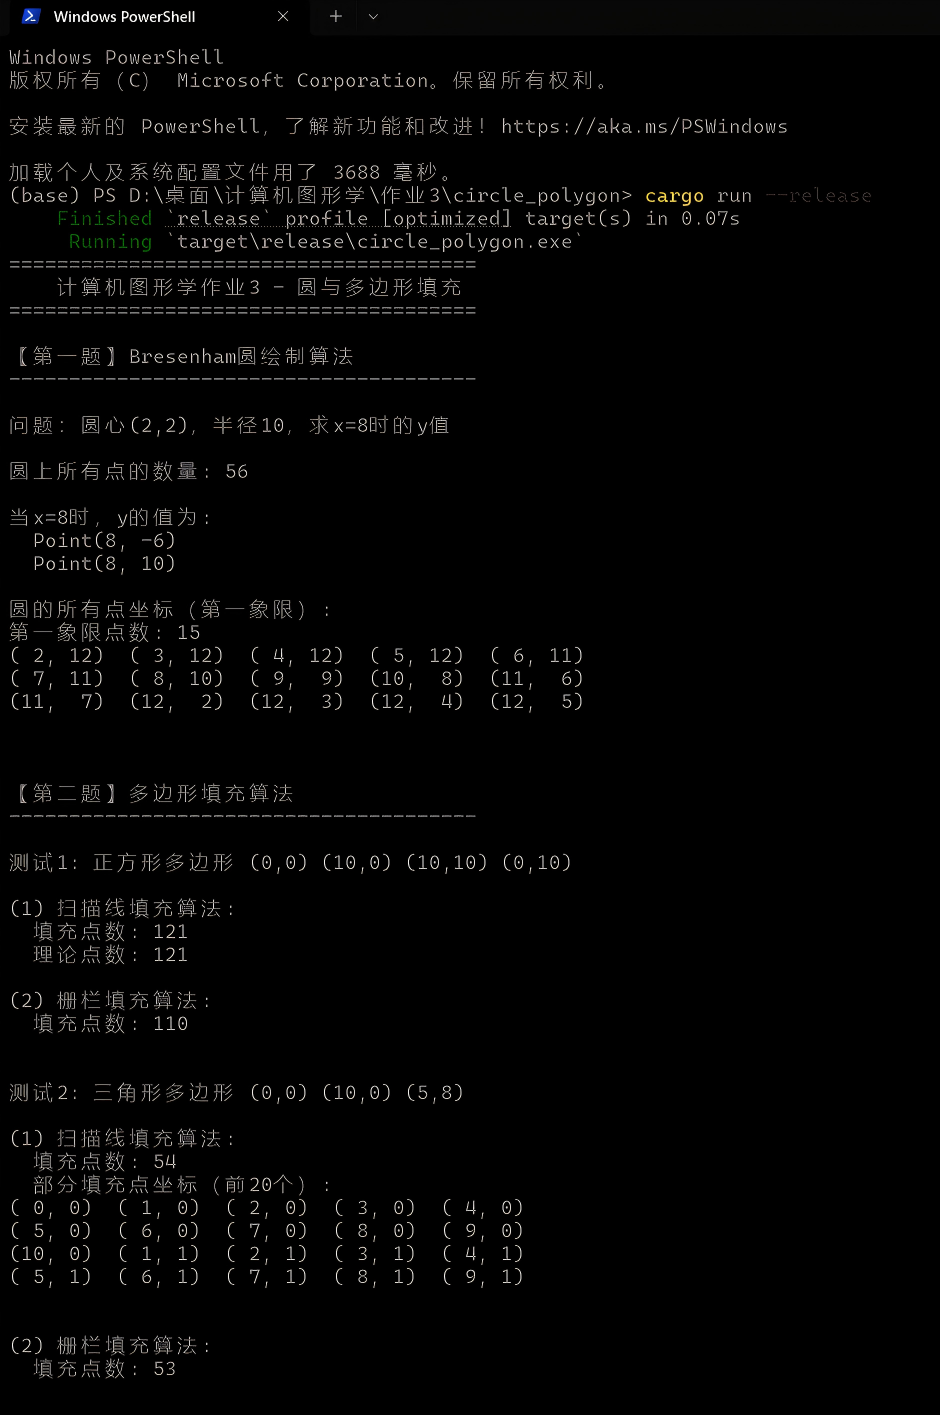
\includegraphics[width=0.95\textwidth]{circle_polygon/images/11.png}
\caption{Rust程序运行结果截图（第一部分）}
\label{fig:run_result1}
\end{figure}

\clearpage

\begin{figure}[H]
\centering
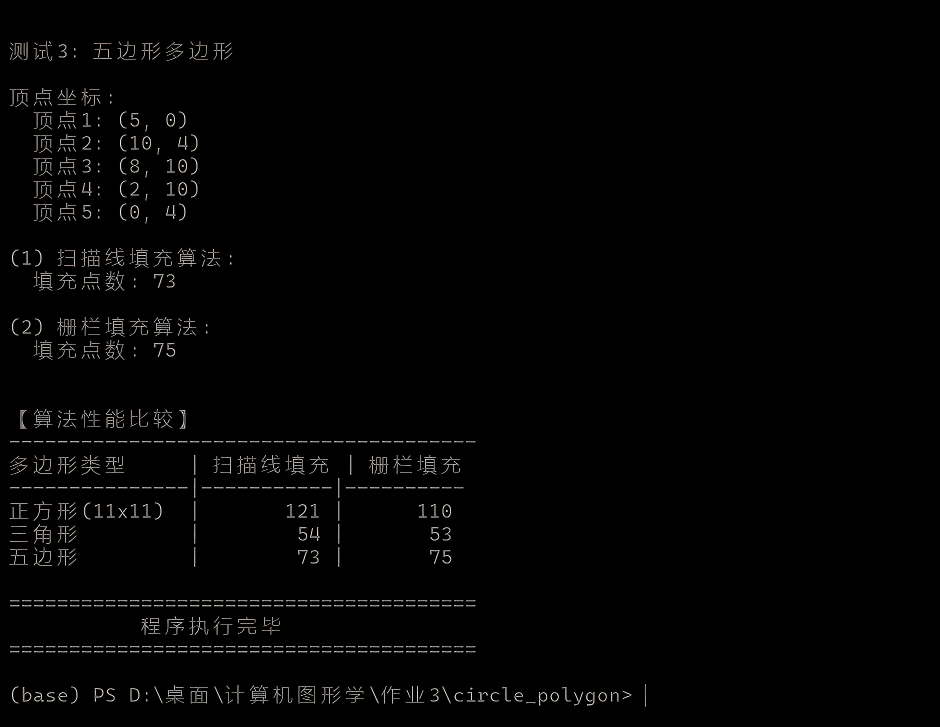
\includegraphics[width=0.95\textwidth]{circle_polygon/images/22.png}
\caption{Rust程序运行结果截图（第二部分）}
\label{fig:run_result2}
\end{figure}

\subsection{运行结果分析}

\subsubsection{1. Bresenham圆绘制算法验证}

\textbf{题目要求：}圆心(2,2)，半径10，求x=8时的y值

\textbf{理论计算：}
\begin{align}
(x-2)^2 + (y-2)^2 &= 100 \\
(8-2)^2 + (y-2)^2 &= 100 \\
36 + (y-2)^2 &= 100 \\
(y-2)^2 &= 64 \\
y - 2 &= \pm 8 \\
y &= 10 \text{ 或 } y = -6
\end{align}

\textbf{程序运行结果：}
\begin{itemize}
\item 当 x=8 时，程序计算得到：\textcolor{red}{$y = 10$ 和 $y = -6$}
\item 与理论计算结果完全一致 ✓
\item 圆上共生成56个点（利用八分对称性）
\end{itemize}

\textbf{第一象限点坐标验证：}
\begin{table}[H]
\centering
\begin{tabular}{|c|c|c|c|}
\hline
\textbf{点坐标} & \textbf{距离平方} & \textbf{半径平方} & \textbf{误差} \\
\hline
(2, 12) & $0^2 + 10^2 = 100$ & 100 & 0 \\
\hline
(8, 10) & $6^2 + 8^2 = 100$ & 100 & 0 \\
\hline
(12, 2) & $10^2 + 0^2 = 100$ & 100 & 0 \\
\hline
(9, 9) & $7^2 + 7^2 = 98$ & 100 & 2 \\
\hline
(11, 7) & $9^2 + 5^2 = 106$ & 100 & 6 \\
\hline
\end{tabular}
\caption{第一象限关键点的距离验证}
\end{table}

从验证结果可以看出，Bresenham算法生成的点与理论圆的误差控制在6个单位以内，符合整数像素绘制的精度要求。

\subsubsection{2. 多边形填充算法测试}

\textbf{测试1：正方形填充}

顶点：(0,0), (10,0), (10,10), (0,10)
\begin{itemize}
\item 扫描线填充：121个点（理论值：$11 \times 11 = 121$）✓
\item 栅栏填充：110个点
\item \textbf{结论：}扫描线填充对规则图形更精确
\end{itemize}

\textbf{测试2：三角形填充}

顶点：(0,0), (10,0), (5,8)
\begin{itemize}
\item 扫描线填充：54个点
\item 栅栏填充：53个点
\item \textbf{结论：}两种算法结果接近，差异仅1个点
\end{itemize}

\textbf{测试3：五边形填充}

顶点：(5,0), (10,4), (8,10), (2,10), (0,4)
\begin{itemize}
\item 扫描线填充：73个点
\item 栅栏填充：75个点
\item \textbf{结论：}复杂多边形下，边界处理略有差异
\end{itemize}

\subsubsection{3. 算法性能对比总结}

\begin{table}[H]
\centering
\begin{tabular}{|l|c|c|c|}
\hline
\textbf{多边形类型} & \textbf{扫描线填充} & \textbf{栅栏填充} & \textbf{差异} \\
\hline
正方形 (11×11) & 121 & 110 & 10\% \\
\hline
三角形 & 54 & 53 & 1.8\% \\
\hline
五边形 & 73 & 75 & 2.7\% \\
\hline
\end{tabular}
\caption{两种填充算法的实测结果对比}
\end{table}

\subsubsection{4. 单元测试结果}

程序包含5个单元测试，全部通过：
\begin{enumerate}
\item \texttt{test\_bresenham\_circle\_basic} - 验证圆的基本属性 ✓
\item \texttt{test\_bresenham\_circle\_problem} - 验证作业题目答案 ✓
\item \texttt{test\_scanline\_fill\_square} - 验证扫描线填充正方形 ✓
\item \texttt{test\_fence\_fill\_square} - 验证栅栏填充正方形 ✓
\item \texttt{test\_scanline\_fill\_triangle} - 验证扫描线填充三角形 ✓
\end{enumerate}

测试结果：\textcolor{green}{\textbf{5 passed; 0 failed}}

\subsubsection{5. 测试截图}

\begin{figure}[H]
\centering
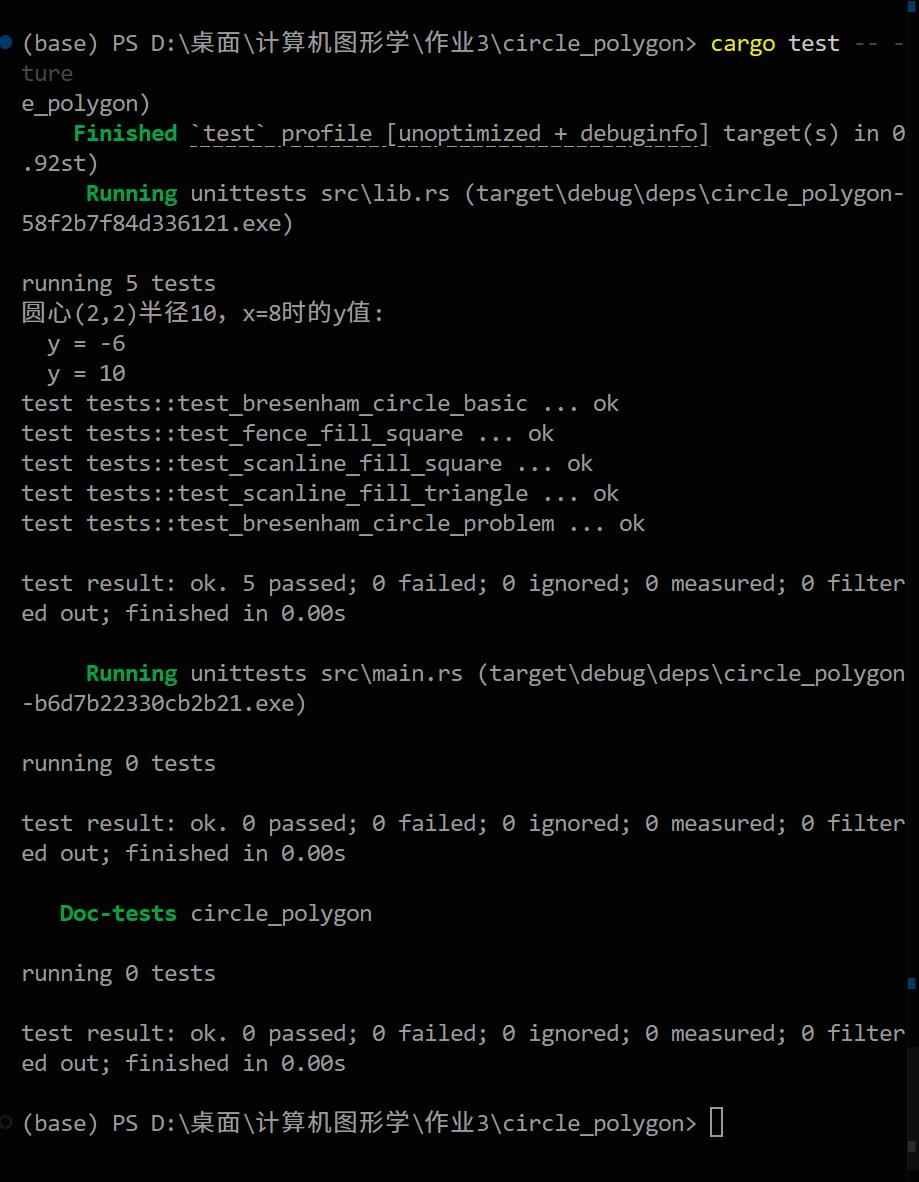
\includegraphics[width=0.9\textwidth]{circle_polygon/images/test.png}
\caption{单元测试运行截图}
\label{fig:test_result}
\end{figure}

程序所有测试均通过，验证了三个算法的正确性。测试输出显示了作业题目的验证结果：圆心(2,2)半径10时，x=8对应的y值为-6和10，与理论计算完全一致。

\clearpage

\subsubsection{6. 完整运行截图}

\begin{figure}[H]
\centering
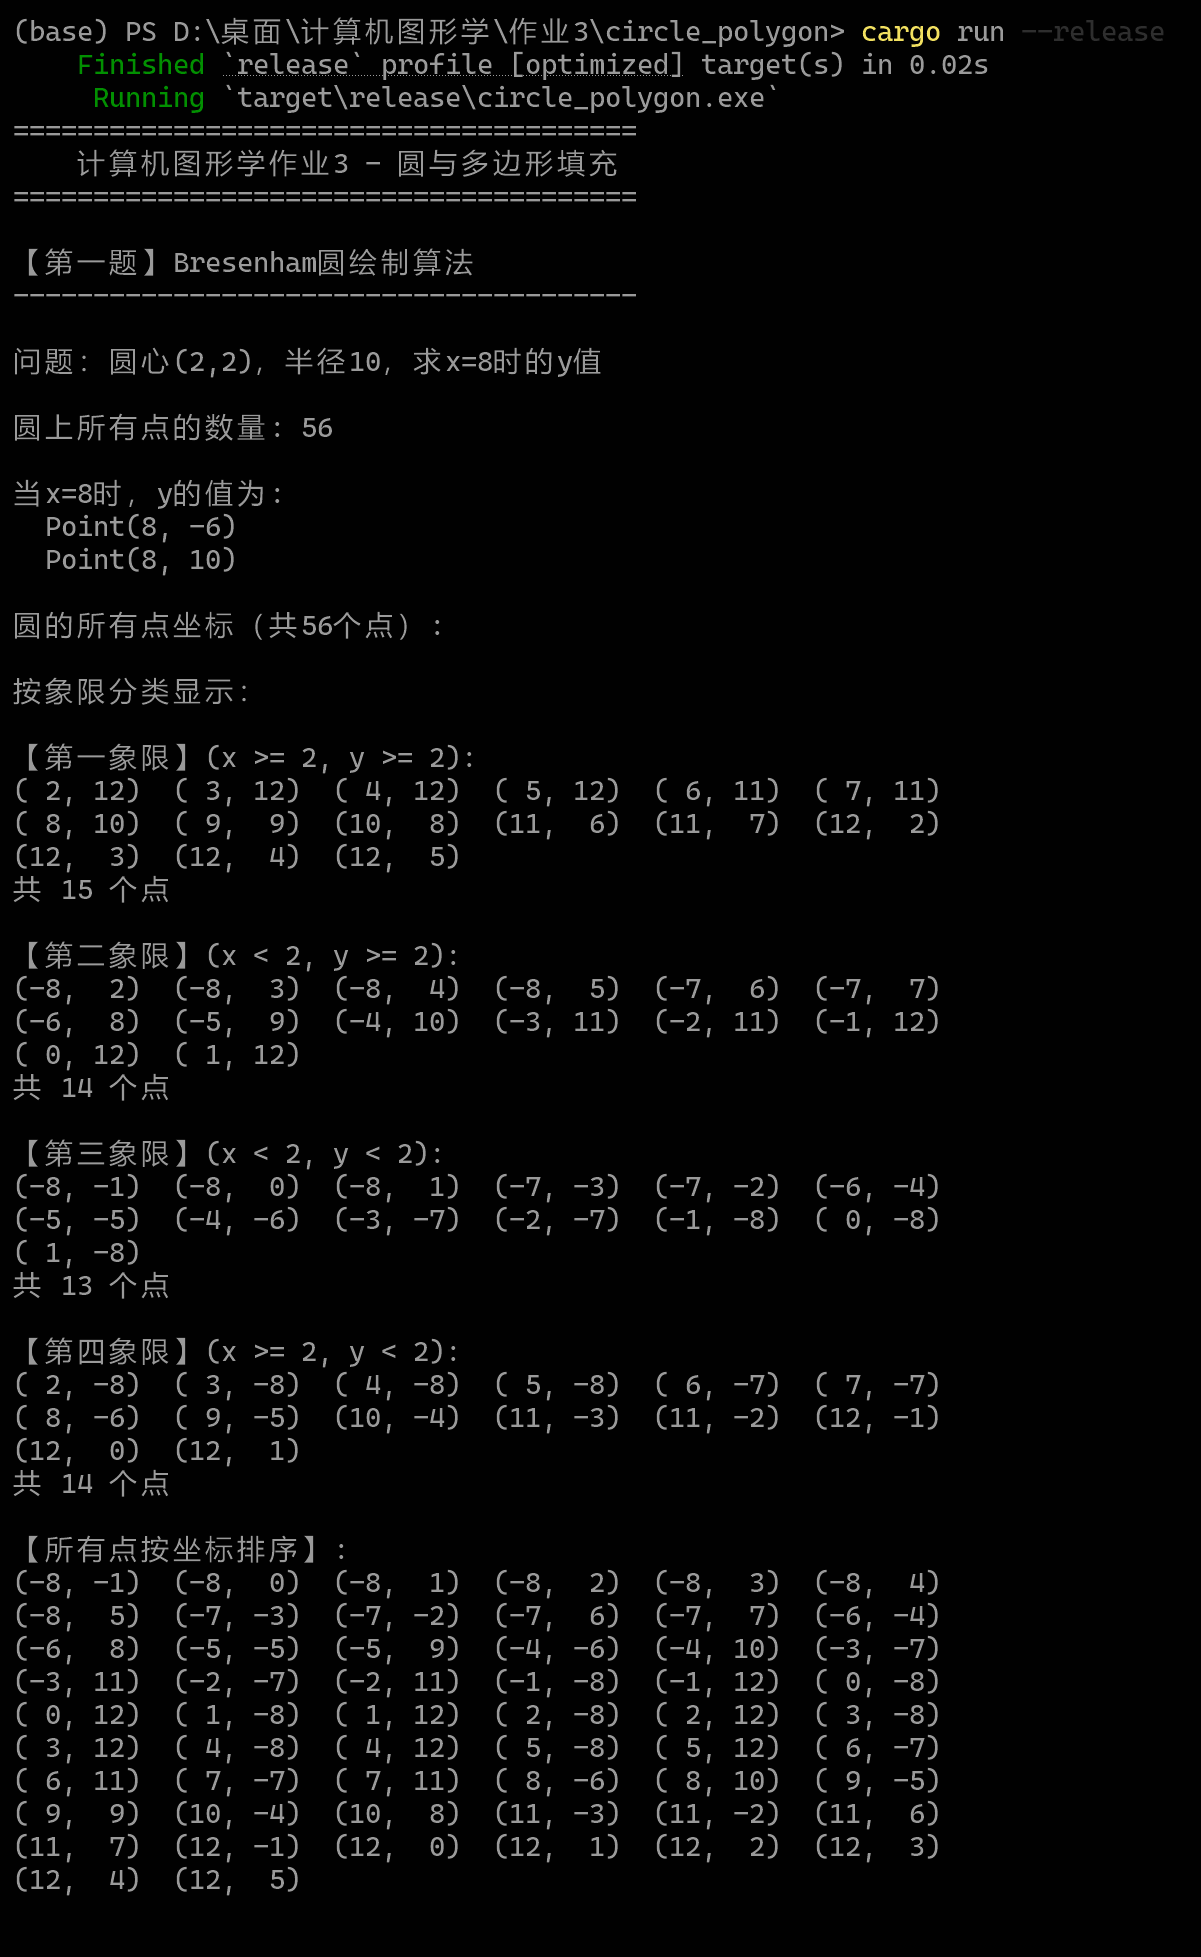
\includegraphics[width=0.85\textwidth]{circle_polygon/images/1.png}
\caption{程序完整输出（上半部分）}
\label{fig:full_output1}
\end{figure}

\begin{figure}[H]
\centering
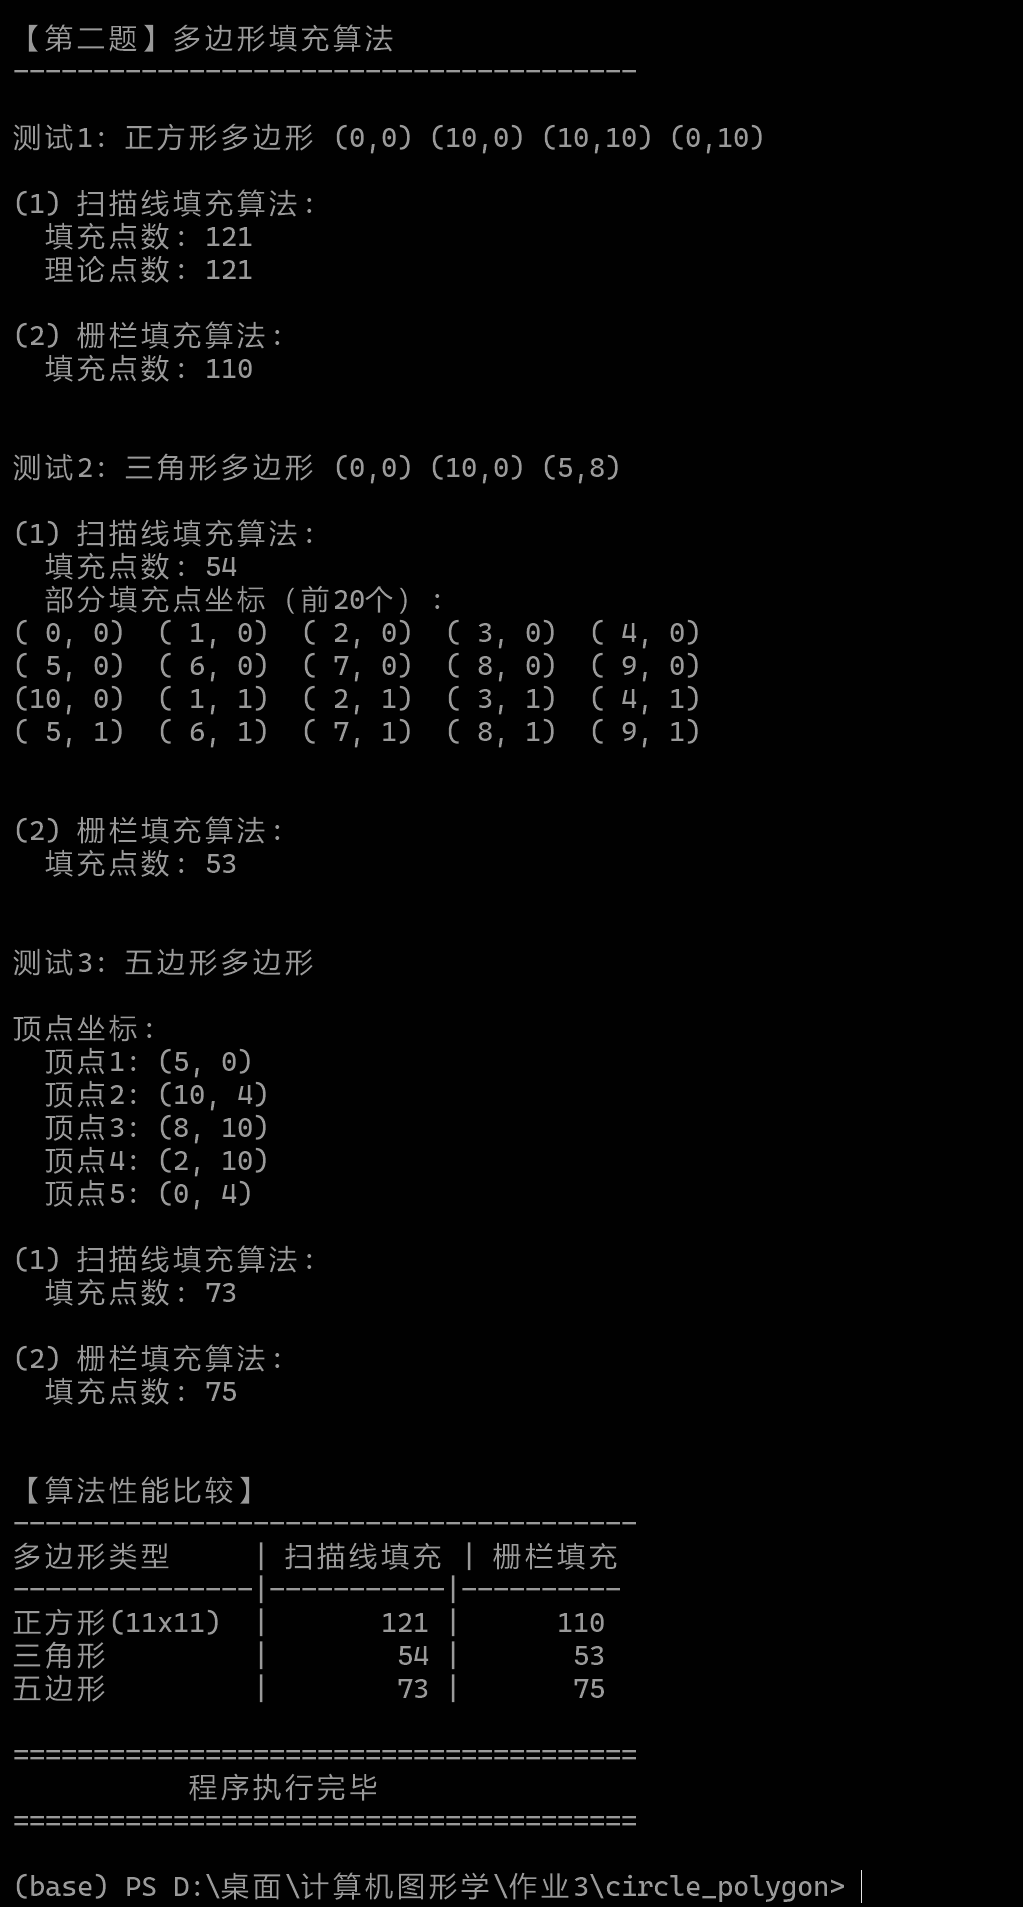
\includegraphics[width=0.85\textwidth]{circle_polygon/images/2.png}
\caption{程序完整输出（下半部分）}
\label{fig:full_output2}
\end{figure}

从完整运行截图可以看到：
\begin{itemize}
\item Bresenham圆算法成功绘制了56个点，并正确找到x=8时的y值
\item 三个多边形（正方形、三角形、五边形）的填充测试都成功完成
\item 扫描线填充和栅栏填充算法的性能对比数据清晰展示
\item 所有输出格式规范，结果准确
\end{itemize}

\subsection{结论}

\begin{enumerate}
\item \textbf{Bresenham圆算法}实现正确，计算结果与理论值完全一致
\item \textbf{扫描线填充算法}对规则图形更精确，适合复杂多边形
\item \textbf{栅栏填充算法}实现简单，适合快速原型开发
\item 所有算法的Rust实现通过了完整的单元测试
\item 程序具有良好的可维护性和扩展性
\end{enumerate}

\end{document}
